\section{Methods}

\subsection{Ecological trait data collection}
I collated ecological trait data for terrestrial vertebrates from published databases and unpublished sources (Table). Targeted traits related to species life history (body mass, longevity, litter or clutch size, trophic level, diet) and to their habitat preferences. Traits were selected for three main reasons: (1) estimates were available for many species; (2) estimates were available across all four terrestrial vertebrate classes, allowing cross-classes comparative analyses (true for all traits except diet); (3) selected traits have been shown to be response or effect traits in other studies or are related to response or effect traits (Table 1, and additional refs). Selecting traits that were ecologically relevant was particularly important, and I will develop this point further down.

All continuous traits were averaged within species when different sources provided estimates. Species diet was described as a binary variable recording whether food items were known to be consumed by a species or not. Diet was available for all classes except reptiles. For amphibians and birds, trophic levels were partly derived from the diet. Species habitat preferences were compiled from IUCN habitat data files and were described as a binary variable recording whether a species was known to occur in a particular habitat. See Supporting Information for details on food items and recorded habitats.

I used these compiled traits to design three other ecological variables. Diet breadth was calculated as the number of food items a species was recorded to ingest. Similarly, habitat breadth was calculated as the number of habitats a species was known to use. Weights were assigned to each habitat in this calculation depending on whether the habitat was recorded to be suitable or marginal for each species (see SI). Finally, a broad degree of habitat specialisation was produced. If any artificial habitat was recorded to be suitable, species were reported to be generalists; else, they were natural habitat specialists.

Due to the lack of comprehensive diet information readily available for reptiles, and despite compilation efforts for other classes, diet was excluded from further analyses in all four classes.

In addition, I compiled traits that were potentially correlated to either body mass or age at sexual maturity, to be used as potential predictors in imputations of missing values. As such, body length information was compiled when available, as well as generation length or age at sexual maturity. Longevity and maximum longevity were assumed to provide the same information and were averaged within species.

Finally, species geographical range sizes were calculated from distribution data, extracted from the IUCN Red List. I obtained phylogenetic trees for birds, amphibians, mammals and squamates from Hedges et al (2015) (available at http://www.biodiversitycenter.org/ttol, downloaded 06/07/2018).

%% Table with sources and trait datasets

\subsection{Taxonomic synonymy}
\subsubsection{Extracting synonyms and harmonising taxonomy in trait datasets.}
Across the different sources, similar species could appear under different binomial names. Taxonomic synonymy created `pseudoreplicates' of the same species, overall falsely increasing the total number of species and artificially inflating the amount of missing trait values. As such, taxonomic synonymy was a major issue; due to the large number of species across datasets, extensive manual checks could not be applied. The presence of typos in species names had the same effect as synonymy. I attempted to correct for taxonomy by developping an automated procedure, complemented with a few manual entries. Obvious cases where vernacular names had been entered in the place of binomial names were also treated manually; when possible, I best assigned binomial names to species common names. 

The automated procedure consisted in extracting species accepted and synonymic binomial names from the IUCN Red List or from the Integrated Taxonomic Information System database (ITIS), using the rredlist and taxize R packages. For each class, I started by generating a list of all binomial names figuring across datasets. These `original' binomial names were corrected for typos using gnr\textunderscore resolve (taxize R package). For each of these corrected names, the IUCN RedList was queried and synonyms and accepted names were stored. When species were not found in the IUCN Red List, information was extracted from ITIS. When species were not found in ITIS either, corrected names were assumed to be accepted. Family and order information was extracted using the same procedure and some entries were completed using the Global Biodiversity Information Facility taxonomic backbone (https://www.gbif.org/tools/species-lookup). Taxonomy across datasets was finally homogenised by replacing recorded synonyms with their accepted scientific names.

Overall, this procedure reduced the total number of species figuring in trait datasets (Table). Nevertheless, additional manual checks were required to make sure that all vertebrate species appearing in PREDICTS were represented in the trait datasets. Taxonomic synonymy was resolved manually for PREDICTS species that did not match any species. After synonyms were manually entered for this set of species, all species in PREDICTS were represented in the trait datasets. This underlines the fact that the automated procedure was not optimal in extracting synonyms; species `pseudoreplication' is likely to have persisted to a degree. 

% Result table: delta number of species 
% Extract of synonym dataset


\subsubsection{Increasing species representation and harmonising taxonomy in phylogenetic trees.}

\paragraph{Random species attachments.} Some species in the trait datasets were not represented in the phylogenies (Table). When applicable, and to increase representation, these species were randomly attached to their genera in the trees (phytools package). Only a small fraction of species that had no phylogenetic position were randomly attached to their genera (Table).

\begin{table}[h!]
\renewcommand{\baselinestretch}{1}
\renewcommand{\arraystretch}{1.5}
\begin{center}\fontsize{9}{11}\selectfont
\caption[Species representation in phylogenetic trees]{\textbf{Species representation in phylogenetic trees.}} 
\label{random_attachments_phy}
\begin{tabular}{|l|l|l|c|l}
\cline{1-4}
\multicolumn{1}{|c|}{Class} & \multicolumn{1}{c|}{No phylogenetic position} & \multicolumn{1}{c|}{Randomly attached} & No representation in tree &  \\ \cline{1-4}
Amphibians                  & 59\% (4062 of 6927)                           & 0.4\% (17 of 4062)                     & \textbf{58\%}             &  \\ \cline{1-4}
Birds                       & 18\% (2084 of 11637)                          & 4.8\% (100 of 2084)                    & \textbf{17\%}             &  \\ \cline{1-4}
Mammals                     & 7.4\% (407 of 5502)                           & 23\% (94 of 407)                       & \textbf{5.7\%}            &  \\ \cline{1-4}
Reptiles                    & 62\% (6391 of 10334)                          & 9.6\% (611 of 6391)                    & \textbf{56\%}             &  \\ \cline{1-4}
\end{tabular}
\end{center}
\end{table}

\paragraph{Taxonomic correction across tip labels.} 
To correct for taxonomy across phylogenies, I applied the same method as above, replacing synonyms by their identified accepted names in trees' tip labels. In some cases, this procedure assigned the same accepted name to different phylogenetic tips. This was the case for 2.6\% of mammalian, 1.5\% of avian, 1\% of amphibian and  1.5\% of reptilian species, which then had multiple phylogenetic positions. In other words, replicated tips appeared. Most of these replicated species had two different positions (see table). For each replicated tip, I selected one tip to conserve and dropped other tips from the phylogenies (see Figure). If replicated tips were sister clades, the tip to conserve was chosen randomly among the replicates. Else, I chose to converse the tree tip whose position was closest to the position of the same tip in the uncorrected tree, when present. In all other few cases, tips to drop were chosen randomly. Further details on how replicated tips were dropped are available in the SI.

\subsection{Trait filtering and transformations}
Species for which all trait values were missing were filtered out. All continuous traits were log10 (except habitat, square root) and standardised to zero-mean and unit variance.


\subsection{Imputation of missing trait values}

\subsubsection{Increase in trait coverage due to taxonomic correction}
The amount of missing values varied importantly across classes and across traits. For birds and mammals, initial trait coverage ranged from XX to XX, whereas for amphibians and reptiles, coverage ranged from XX to XX. 

\begin{figure}[h!]
\centering
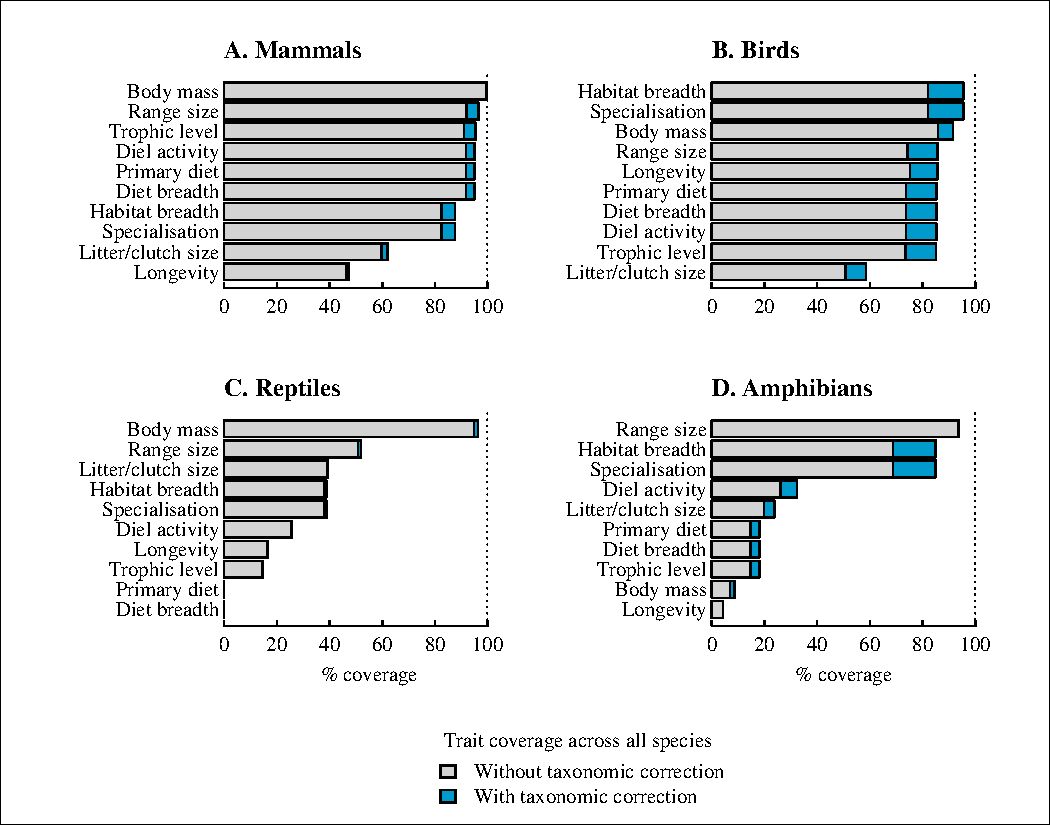
\includegraphics[scale=0.85]{figures/chapter2/Target_traits_All_species_coverage}
\caption[Trait coverage across all species before and after taxonomic correction]{\textbf{Trait coverage across all species before and after taxonomic correction.} Trait coverage is defined here as the percentage of species for which trait information is available. Correcting for taxonomic synonymy improved trait coverage in most cases.}
\end{figure}

\begin{figure}[h!]
\centering
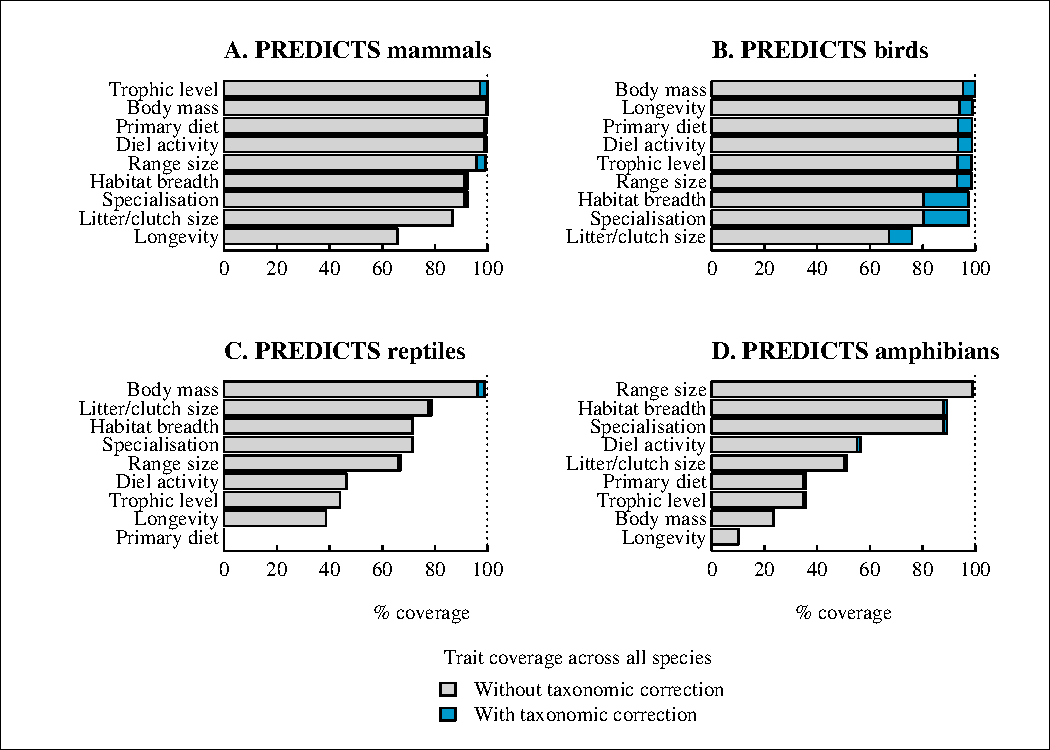
\includegraphics[scale=0.85]{figures/chapter2/Target_traits_Predicts_species_coverage}
\caption[Trait coverage across PREDICTS species before and after taxonomic correction]{\textbf{Trait coverage across all species before and after taxonomic correction.} Trait coverage is defined here as the percentage of species for which trait information is available. Correcting for taxonomic synonymy improved trait coverage in most cases.}
\end{figure}


\subsubsection{Species representation in phylogenetic trees}
\begin{figure}[h!]
\centering
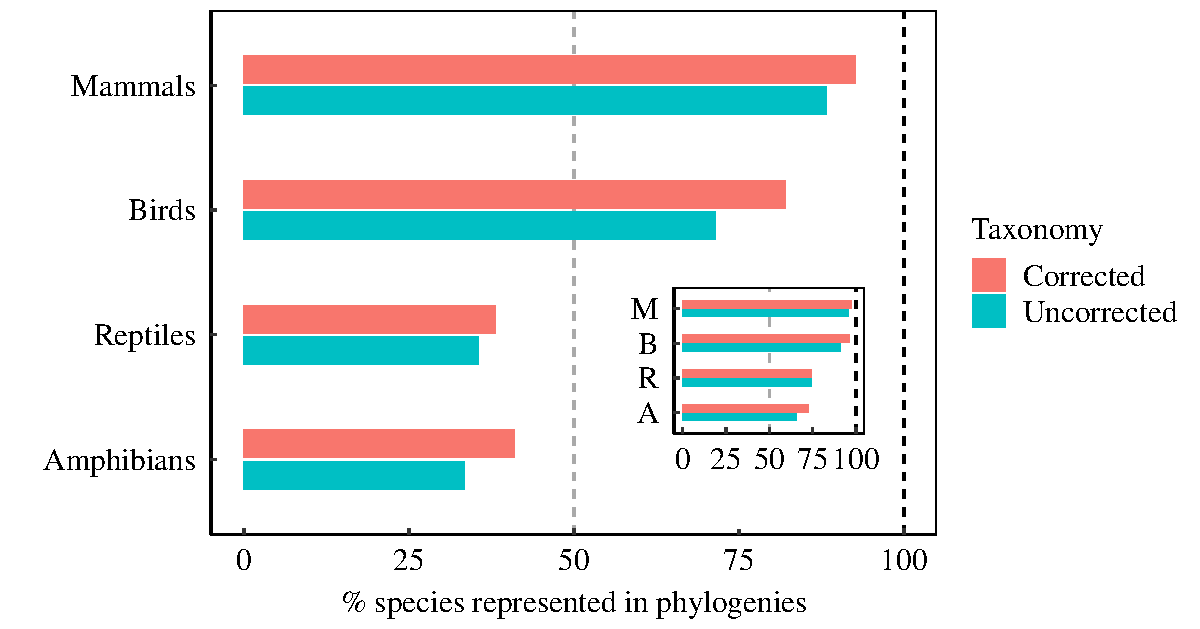
\includegraphics[scale=0.7]{figures/chapter2/Species_representation_phylo}
\caption[Percentage of species represented in the phylogenies for both corrected and uncorrected trait datasets]{\textbf{Percentage of species represented in the phylogenies for both corrected and uncorrected trait datasets.} Overall, taxonomic correction increased species representation in phylogenetic trees. Representation for mammals and birds was high (after correction: 83\% of avian and 94\% of mammalian species had a phylogenetic position). On the other hand, reptiles and amphibians were poorly represented (after correction: only 39\% of reptilian and 42\% of amphibian species were placed in phylogenetic trees). The inset barplot shows representation for species figuring in PREDICTS. For these, species presence in phylogenetic trees after correction was high across all classes, with a minimum representation of 73\% for amphibians.}
\end{figure}

\subsubsection{Randomness in missing trait values}

\subsubsection{Phylogenetic signal}

\subsubsection{Imputations of missing trait values}

I imputed missing values using random forest algorithms (missForest R package). For some traits, the phylogenetic signal (assessed using Pagel’s lambda) was strong, showing that they were highly evolutionary conserved. To account for phylogenetic relationships among species, phylogenetic eigenvectors were included in the random forest imputations as a supplementary predictor. Eigenvectors were extracted from the phylogenies using the PVR package (Santos, 2018). Penone et al showed that including 10 eigenvectors minimised the imputation errors – hence I included 10 eigenvectors. Plus best method with phylogenies.

Otherwise, traits for these sets of species were imputed without additional phylogenetic information, in a second round of imputations, with family, order, and genus as additional predictors.

Robustness of imputations

\section{Results}


\section{Discussion}
Discuss taxonomy and robustness of imputations

